\documentclass{article}



\usepackage{iclr2022/iclr2022_conference,times}

% Optional math commands from https://github.com/goodfeli/dlbook_notation.
%%%%% NEW MATH DEFINITIONS %%%%%

\usepackage{amsmath,amsfonts,bm}

% Mark sections of captions for referring to divisions of figures
\newcommand{\figleft}{{\em (Left)}}
\newcommand{\figcenter}{{\em (Center)}}
\newcommand{\figright}{{\em (Right)}}
\newcommand{\figtop}{{\em (Top)}}
\newcommand{\figbottom}{{\em (Bottom)}}
\newcommand{\captiona}{{\em (a)}}
\newcommand{\captionb}{{\em (b)}}
\newcommand{\captionc}{{\em (c)}}
\newcommand{\captiond}{{\em (d)}}

% Highlight a newly defined term
\newcommand{\newterm}[1]{{\bf #1}}


% Figure reference, lower-case.
\def\figref#1{figure~\ref{#1}}
% Figure reference, capital. For start of sentence
\def\Figref#1{Figure~\ref{#1}}
\def\twofigref#1#2{figures \ref{#1} and \ref{#2}}
\def\quadfigref#1#2#3#4{figures \ref{#1}, \ref{#2}, \ref{#3} and \ref{#4}}
% Section reference, lower-case.
\def\secref#1{section~\ref{#1}}
% Section reference, capital.
\def\Secref#1{Section~\ref{#1}}
% Reference to two sections.
\def\twosecrefs#1#2{sections \ref{#1} and \ref{#2}}
% Reference to three sections.
\def\secrefs#1#2#3{sections \ref{#1}, \ref{#2} and \ref{#3}}
% Reference to an equation, lower-case.
\def\eqref#1{equation~\ref{#1}}
% Reference to an equation, upper case
\def\Eqref#1{Equation~\ref{#1}}
% A raw reference to an equation---avoid using if possible
\def\plaineqref#1{\ref{#1}}
% Reference to a chapter, lower-case.
\def\chapref#1{chapter~\ref{#1}}
% Reference to an equation, upper case.
\def\Chapref#1{Chapter~\ref{#1}}
% Reference to a range of chapters
\def\rangechapref#1#2{chapters\ref{#1}--\ref{#2}}
% Reference to an algorithm, lower-case.
\def\algref#1{algorithm~\ref{#1}}
% Reference to an algorithm, upper case.
\def\Algref#1{Algorithm~\ref{#1}}
\def\twoalgref#1#2{algorithms \ref{#1} and \ref{#2}}
\def\Twoalgref#1#2{Algorithms \ref{#1} and \ref{#2}}
% Reference to a part, lower case
\def\partref#1{part~\ref{#1}}
% Reference to a part, upper case
\def\Partref#1{Part~\ref{#1}}
\def\twopartref#1#2{parts \ref{#1} and \ref{#2}}

\def\ceil#1{\lceil #1 \rceil}
\def\floor#1{\lfloor #1 \rfloor}
\def\1{\bm{1}}
\newcommand{\train}{\mathcal{D}}
\newcommand{\valid}{\mathcal{D_{\mathrm{valid}}}}
\newcommand{\test}{\mathcal{D_{\mathrm{test}}}}

\def\eps{{\epsilon}}


% Random variables
\def\reta{{\textnormal{$\eta$}}}
\def\ra{{\textnormal{a}}}
\def\rb{{\textnormal{b}}}
\def\rc{{\textnormal{c}}}
\def\rd{{\textnormal{d}}}
\def\re{{\textnormal{e}}}
\def\rf{{\textnormal{f}}}
\def\rg{{\textnormal{g}}}
\def\rh{{\textnormal{h}}}
\def\ri{{\textnormal{i}}}
\def\rj{{\textnormal{j}}}
\def\rk{{\textnormal{k}}}
\def\rl{{\textnormal{l}}}
% rm is already a command, just don't name any random variables m
\def\rn{{\textnormal{n}}}
\def\ro{{\textnormal{o}}}
\def\rp{{\textnormal{p}}}
\def\rq{{\textnormal{q}}}
\def\rr{{\textnormal{r}}}
\def\rs{{\textnormal{s}}}
\def\rt{{\textnormal{t}}}
\def\ru{{\textnormal{u}}}
\def\rv{{\textnormal{v}}}
\def\rw{{\textnormal{w}}}
\def\rx{{\textnormal{x}}}
\def\ry{{\textnormal{y}}}
\def\rz{{\textnormal{z}}}

% Random vectors
\def\rvepsilon{{\mathbf{\epsilon}}}
\def\rvtheta{{\mathbf{\theta}}}
\def\rva{{\mathbf{a}}}
\def\rvb{{\mathbf{b}}}
\def\rvc{{\mathbf{c}}}
\def\rvd{{\mathbf{d}}}
\def\rve{{\mathbf{e}}}
\def\rvf{{\mathbf{f}}}
\def\rvg{{\mathbf{g}}}
\def\rvh{{\mathbf{h}}}
\def\rvu{{\mathbf{i}}}
\def\rvj{{\mathbf{j}}}
\def\rvk{{\mathbf{k}}}
\def\rvl{{\mathbf{l}}}
\def\rvm{{\mathbf{m}}}
\def\rvn{{\mathbf{n}}}
\def\rvo{{\mathbf{o}}}
\def\rvp{{\mathbf{p}}}
\def\rvq{{\mathbf{q}}}
\def\rvr{{\mathbf{r}}}
\def\rvs{{\mathbf{s}}}
\def\rvt{{\mathbf{t}}}
\def\rvu{{\mathbf{u}}}
\def\rvv{{\mathbf{v}}}
\def\rvw{{\mathbf{w}}}
\def\rvx{{\mathbf{x}}}
\def\rvy{{\mathbf{y}}}
\def\rvz{{\mathbf{z}}}

% Elements of random vectors
\def\erva{{\textnormal{a}}}
\def\ervb{{\textnormal{b}}}
\def\ervc{{\textnormal{c}}}
\def\ervd{{\textnormal{d}}}
\def\erve{{\textnormal{e}}}
\def\ervf{{\textnormal{f}}}
\def\ervg{{\textnormal{g}}}
\def\ervh{{\textnormal{h}}}
\def\ervi{{\textnormal{i}}}
\def\ervj{{\textnormal{j}}}
\def\ervk{{\textnormal{k}}}
\def\ervl{{\textnormal{l}}}
\def\ervm{{\textnormal{m}}}
\def\ervn{{\textnormal{n}}}
\def\ervo{{\textnormal{o}}}
\def\ervp{{\textnormal{p}}}
\def\ervq{{\textnormal{q}}}
\def\ervr{{\textnormal{r}}}
\def\ervs{{\textnormal{s}}}
\def\ervt{{\textnormal{t}}}
\def\ervu{{\textnormal{u}}}
\def\ervv{{\textnormal{v}}}
\def\ervw{{\textnormal{w}}}
\def\ervx{{\textnormal{x}}}
\def\ervy{{\textnormal{y}}}
\def\ervz{{\textnormal{z}}}

% Random matrices
\def\rmA{{\mathbf{A}}}
\def\rmB{{\mathbf{B}}}
\def\rmC{{\mathbf{C}}}
\def\rmD{{\mathbf{D}}}
\def\rmE{{\mathbf{E}}}
\def\rmF{{\mathbf{F}}}
\def\rmG{{\mathbf{G}}}
\def\rmH{{\mathbf{H}}}
\def\rmI{{\mathbf{I}}}
\def\rmJ{{\mathbf{J}}}
\def\rmK{{\mathbf{K}}}
\def\rmL{{\mathbf{L}}}
\def\rmM{{\mathbf{M}}}
\def\rmN{{\mathbf{N}}}
\def\rmO{{\mathbf{O}}}
\def\rmP{{\mathbf{P}}}
\def\rmQ{{\mathbf{Q}}}
\def\rmR{{\mathbf{R}}}
\def\rmS{{\mathbf{S}}}
\def\rmT{{\mathbf{T}}}
\def\rmU{{\mathbf{U}}}
\def\rmV{{\mathbf{V}}}
\def\rmW{{\mathbf{W}}}
\def\rmX{{\mathbf{X}}}
\def\rmY{{\mathbf{Y}}}
\def\rmZ{{\mathbf{Z}}}

% Elements of random matrices
\def\ermA{{\textnormal{A}}}
\def\ermB{{\textnormal{B}}}
\def\ermC{{\textnormal{C}}}
\def\ermD{{\textnormal{D}}}
\def\ermE{{\textnormal{E}}}
\def\ermF{{\textnormal{F}}}
\def\ermG{{\textnormal{G}}}
\def\ermH{{\textnormal{H}}}
\def\ermI{{\textnormal{I}}}
\def\ermJ{{\textnormal{J}}}
\def\ermK{{\textnormal{K}}}
\def\ermL{{\textnormal{L}}}
\def\ermM{{\textnormal{M}}}
\def\ermN{{\textnormal{N}}}
\def\ermO{{\textnormal{O}}}
\def\ermP{{\textnormal{P}}}
\def\ermQ{{\textnormal{Q}}}
\def\ermR{{\textnormal{R}}}
\def\ermS{{\textnormal{S}}}
\def\ermT{{\textnormal{T}}}
\def\ermU{{\textnormal{U}}}
\def\ermV{{\textnormal{V}}}
\def\ermW{{\textnormal{W}}}
\def\ermX{{\textnormal{X}}}
\def\ermY{{\textnormal{Y}}}
\def\ermZ{{\textnormal{Z}}}

% Vectors
\def\vzero{{\bm{0}}}
\def\vone{{\bm{1}}}
\def\vmu{{\bm{\mu}}}
\def\vtheta{{\bm{\theta}}}
\def\va{{\bm{a}}}
\def\vb{{\bm{b}}}
\def\vc{{\bm{c}}}
\def\vd{{\bm{d}}}
\def\ve{{\bm{e}}}
\def\vf{{\bm{f}}}
\def\vg{{\bm{g}}}
\def\vh{{\bm{h}}}
\def\vi{{\bm{i}}}
\def\vj{{\bm{j}}}
\def\vk{{\bm{k}}}
\def\vl{{\bm{l}}}
\def\vm{{\bm{m}}}
\def\vn{{\bm{n}}}
\def\vo{{\bm{o}}}
\def\vp{{\bm{p}}}
\def\vq{{\bm{q}}}
\def\vr{{\bm{r}}}
\def\vs{{\bm{s}}}
\def\vt{{\bm{t}}}
\def\vu{{\bm{u}}}
\def\vv{{\bm{v}}}
\def\vw{{\bm{w}}}
\def\vx{{\bm{x}}}
\def\vy{{\bm{y}}}
\def\vz{{\bm{z}}}

% Elements of vectors
\def\evalpha{{\alpha}}
\def\evbeta{{\beta}}
\def\evepsilon{{\epsilon}}
\def\evlambda{{\lambda}}
\def\evomega{{\omega}}
\def\evmu{{\mu}}
\def\evpsi{{\psi}}
\def\evsigma{{\sigma}}
\def\evtheta{{\theta}}
\def\eva{{a}}
\def\evb{{b}}
\def\evc{{c}}
\def\evd{{d}}
\def\eve{{e}}
\def\evf{{f}}
\def\evg{{g}}
\def\evh{{h}}
\def\evi{{i}}
\def\evj{{j}}
\def\evk{{k}}
\def\evl{{l}}
\def\evm{{m}}
\def\evn{{n}}
\def\evo{{o}}
\def\evp{{p}}
\def\evq{{q}}
\def\evr{{r}}
\def\evs{{s}}
\def\evt{{t}}
\def\evu{{u}}
\def\evv{{v}}
\def\evw{{w}}
\def\evx{{x}}
\def\evy{{y}}
\def\evz{{z}}

% Matrix
\def\mA{{\bm{A}}}
\def\mB{{\bm{B}}}
\def\mC{{\bm{C}}}
\def\mD{{\bm{D}}}
\def\mE{{\bm{E}}}
\def\mF{{\bm{F}}}
\def\mG{{\bm{G}}}
\def\mH{{\bm{H}}}
\def\mI{{\bm{I}}}
\def\mJ{{\bm{J}}}
\def\mK{{\bm{K}}}
\def\mL{{\bm{L}}}
\def\mM{{\bm{M}}}
\def\mN{{\bm{N}}}
\def\mO{{\bm{O}}}
\def\mP{{\bm{P}}}
\def\mQ{{\bm{Q}}}
\def\mR{{\bm{R}}}
\def\mS{{\bm{S}}}
\def\mT{{\bm{T}}}
\def\mU{{\bm{U}}}
\def\mV{{\bm{V}}}
\def\mW{{\bm{W}}}
\def\mX{{\bm{X}}}
\def\mY{{\bm{Y}}}
\def\mZ{{\bm{Z}}}
\def\mBeta{{\bm{\beta}}}
\def\mPhi{{\bm{\Phi}}}
\def\mLambda{{\bm{\Lambda}}}
\def\mSigma{{\bm{\Sigma}}}

% Tensor
\DeclareMathAlphabet{\mathsfit}{\encodingdefault}{\sfdefault}{m}{sl}
\SetMathAlphabet{\mathsfit}{bold}{\encodingdefault}{\sfdefault}{bx}{n}
\newcommand{\tens}[1]{\bm{\mathsfit{#1}}}
\def\tA{{\tens{A}}}
\def\tB{{\tens{B}}}
\def\tC{{\tens{C}}}
\def\tD{{\tens{D}}}
\def\tE{{\tens{E}}}
\def\tF{{\tens{F}}}
\def\tG{{\tens{G}}}
\def\tH{{\tens{H}}}
\def\tI{{\tens{I}}}
\def\tJ{{\tens{J}}}
\def\tK{{\tens{K}}}
\def\tL{{\tens{L}}}
\def\tM{{\tens{M}}}
\def\tN{{\tens{N}}}
\def\tO{{\tens{O}}}
\def\tP{{\tens{P}}}
\def\tQ{{\tens{Q}}}
\def\tR{{\tens{R}}}
\def\tS{{\tens{S}}}
\def\tT{{\tens{T}}}
\def\tU{{\tens{U}}}
\def\tV{{\tens{V}}}
\def\tW{{\tens{W}}}
\def\tX{{\tens{X}}}
\def\tY{{\tens{Y}}}
\def\tZ{{\tens{Z}}}


% Graph
\def\gA{{\mathcal{A}}}
\def\gB{{\mathcal{B}}}
\def\gC{{\mathcal{C}}}
\def\gD{{\mathcal{D}}}
\def\gE{{\mathcal{E}}}
\def\gF{{\mathcal{F}}}
\def\gG{{\mathcal{G}}}
\def\gH{{\mathcal{H}}}
\def\gI{{\mathcal{I}}}
\def\gJ{{\mathcal{J}}}
\def\gK{{\mathcal{K}}}
\def\gL{{\mathcal{L}}}
\def\gM{{\mathcal{M}}}
\def\gN{{\mathcal{N}}}
\def\gO{{\mathcal{O}}}
\def\gP{{\mathcal{P}}}
\def\gQ{{\mathcal{Q}}}
\def\gR{{\mathcal{R}}}
\def\gS{{\mathcal{S}}}
\def\gT{{\mathcal{T}}}
\def\gU{{\mathcal{U}}}
\def\gV{{\mathcal{V}}}
\def\gW{{\mathcal{W}}}
\def\gX{{\mathcal{X}}}
\def\gY{{\mathcal{Y}}}
\def\gZ{{\mathcal{Z}}}

% Sets
\def\sA{{\mathbb{A}}}
\def\sB{{\mathbb{B}}}
\def\sC{{\mathbb{C}}}
\def\sD{{\mathbb{D}}}
% Don't use a set called E, because this would be the same as our symbol
% for expectation.
\def\sF{{\mathbb{F}}}
\def\sG{{\mathbb{G}}}
\def\sH{{\mathbb{H}}}
\def\sI{{\mathbb{I}}}
\def\sJ{{\mathbb{J}}}
\def\sK{{\mathbb{K}}}
\def\sL{{\mathbb{L}}}
\def\sM{{\mathbb{M}}}
\def\sN{{\mathbb{N}}}
\def\sO{{\mathbb{O}}}
\def\sP{{\mathbb{P}}}
\def\sQ{{\mathbb{Q}}}
\def\sR{{\mathbb{R}}}
\def\sS{{\mathbb{S}}}
\def\sT{{\mathbb{T}}}
\def\sU{{\mathbb{U}}}
\def\sV{{\mathbb{V}}}
\def\sW{{\mathbb{W}}}
\def\sX{{\mathbb{X}}}
\def\sY{{\mathbb{Y}}}
\def\sZ{{\mathbb{Z}}}

% Entries of a matrix
\def\emLambda{{\Lambda}}
\def\emA{{A}}
\def\emB{{B}}
\def\emC{{C}}
\def\emD{{D}}
\def\emE{{E}}
\def\emF{{F}}
\def\emG{{G}}
\def\emH{{H}}
\def\emI{{I}}
\def\emJ{{J}}
\def\emK{{K}}
\def\emL{{L}}
\def\emM{{M}}
\def\emN{{N}}
\def\emO{{O}}
\def\emP{{P}}
\def\emQ{{Q}}
\def\emR{{R}}
\def\emS{{S}}
\def\emT{{T}}
\def\emU{{U}}
\def\emV{{V}}
\def\emW{{W}}
\def\emX{{X}}
\def\emY{{Y}}
\def\emZ{{Z}}
\def\emSigma{{\Sigma}}

% entries of a tensor
% Same font as tensor, without \bm wrapper
\newcommand{\etens}[1]{\mathsfit{#1}}
\def\etLambda{{\etens{\Lambda}}}
\def\etA{{\etens{A}}}
\def\etB{{\etens{B}}}
\def\etC{{\etens{C}}}
\def\etD{{\etens{D}}}
\def\etE{{\etens{E}}}
\def\etF{{\etens{F}}}
\def\etG{{\etens{G}}}
\def\etH{{\etens{H}}}
\def\etI{{\etens{I}}}
\def\etJ{{\etens{J}}}
\def\etK{{\etens{K}}}
\def\etL{{\etens{L}}}
\def\etM{{\etens{M}}}
\def\etN{{\etens{N}}}
\def\etO{{\etens{O}}}
\def\etP{{\etens{P}}}
\def\etQ{{\etens{Q}}}
\def\etR{{\etens{R}}}
\def\etS{{\etens{S}}}
\def\etT{{\etens{T}}}
\def\etU{{\etens{U}}}
\def\etV{{\etens{V}}}
\def\etW{{\etens{W}}}
\def\etX{{\etens{X}}}
\def\etY{{\etens{Y}}}
\def\etZ{{\etens{Z}}}

% The true underlying data generating distribution
\newcommand{\pdata}{p_{\rm{data}}}
% The empirical distribution defined by the training set
\newcommand{\ptrain}{\hat{p}_{\rm{data}}}
\newcommand{\Ptrain}{\hat{P}_{\rm{data}}}
% The model distribution
\newcommand{\pmodel}{p_{\rm{model}}}
\newcommand{\Pmodel}{P_{\rm{model}}}
\newcommand{\ptildemodel}{\tilde{p}_{\rm{model}}}
% Stochastic autoencoder distributions
\newcommand{\pencode}{p_{\rm{encoder}}}
\newcommand{\pdecode}{p_{\rm{decoder}}}
\newcommand{\precons}{p_{\rm{reconstruct}}}

\newcommand{\laplace}{\mathrm{Laplace}} % Laplace distribution

\newcommand{\E}{\mathbb{E}}
\newcommand{\Ls}{\mathcal{L}}
\newcommand{\R}{\mathbb{R}}
\newcommand{\emp}{\tilde{p}}
\newcommand{\lr}{\alpha}
\newcommand{\reg}{\lambda}
\newcommand{\rect}{\mathrm{rectifier}}
\newcommand{\softmax}{\mathrm{softmax}}
\newcommand{\sigmoid}{\sigma}
\newcommand{\softplus}{\zeta}
\newcommand{\KL}{D_{\mathrm{KL}}}
\newcommand{\Var}{\mathrm{Var}}
\newcommand{\standarderror}{\mathrm{SE}}
\newcommand{\Cov}{\mathrm{Cov}}
% Wolfram Mathworld says $L^2$ is for function spaces and $\ell^2$ is for vectors
% But then they seem to use $L^2$ for vectors throughout the site, and so does
% wikipedia.
\newcommand{\normlzero}{L^0}
\newcommand{\normlone}{L^1}
\newcommand{\normltwo}{L^2}
\newcommand{\normlp}{L^p}
\newcommand{\normmax}{L^\infty}

\newcommand{\parents}{Pa} % See usage in notation.tex. Chosen to match Daphne's book.

\DeclareMathOperator*{\argmax}{arg\,max}
\DeclareMathOperator*{\argmin}{arg\,min}

\DeclareMathOperator{\sign}{sign}
\DeclareMathOperator{\Tr}{Tr}
\let\ab\allowbreak


\usepackage{graphicx}
\usepackage{hyperref}
\usepackage{url}
\usepackage{cleveref}
\usepackage{float}

\title{COMP6258 Reproducibility Report \\ ShuffleMixer}

% Authors must not appear in the submitted version. They should be hidden
% as long as the \iclrfinalcopy macro remains commented out below.
% Non-anonymous submissions will be rejected without review.

\author{Jos-Elliot Jeapes \& Samsom Yebio \\
\texttt{\{jej1g19,sy1c20\}@soton.ac.uk} \\
}



% The \author macro works with any number of authors. There are two commands
% used to separate the names and addresses of multiple authors: \And and \AND.
%
% Using \And between authors leaves it to \LaTeX{} to determine where to break
% the lines. Using \AND forces a linebreak at that point. So, if \LaTeX{}
% puts 3 of 4 authors names on the first line, and the last on the second
% line, try using \AND instead of \And before the third author name.

\newcommand{\fix}{\marginpar{FIX}}
\newcommand{\new}{\marginpar{NEW}}

\iclrfinalcopy % Uncomment for camera-ready version, but NOT for submission.
\begin{document}

    \maketitle

    \begin{abstract}
    This report evaluates the reproducibility of \citet{sun2022shufflemixer}. This was done by attempting to reimplement the model from the information given in the paper, and looking at the output of this new model as well as a pretrained model. The paper is found to be highly reproducible, with the new implementation producing similar results.
    \end{abstract}

    \section{Introduction}

    This reproducibility report focuses on the paper `ShuffleMixer: An Efficient ConvNet for Image
    Super-Resolution by' \citet{sun2022shufflemixer}. It applies techniques from \citet{ma2018shufflenet} to image upsampling, to produce high-quality upsampled images efficiently. The paper describes a set of models: two families (tiny and standard) that can have different upsample factors (2x, 4x). This report focuses on the most impressive, the standard 4x model.

    \subsection{Target Questions} \label{sec:target questions}

    The target questions of this report are:

    \begin{itemize}
        \item Does the model perform as expected when presented with new data?
        \item Can a model with the same architecture and performance be trained:
        \begin{enumerate}
            \item Using just the paper and references as a guide?
            \item With reference to the open-source code?
        \end{enumerate}
    \end{itemize}

    In answer to the above, (1) would show stronger reproducibility than (2). Reproducible aspects of the paper not covered by this report include:

    \begin{itemize}
        \item Complexity and performance compared to competing models,
        \item Comparison of how model parameters effect performance,
        \item Effectiveness of the novel aspects of the model. 
    \end{itemize}

    The first seems outside the scope of this report; it would also be testing the reproducibility of other papers. The others both require multiple training runs of a large model (and so a very large amount of time), and would be uninteresting if the target questions don't show reproducibility.

    \subsection{Methodology}

    Two separate methodologies are used, one for both of the target questions. The first is an attempted reimplementation of the model using just the literature as guidance. The second is running the pretrained model on new data, and comparing the output to the expected results. The reimplemented model is also included in this second comparison, and checked against the original code.

    \section{Reimplementation} \label{sec: reimpl}

    The original paper includes a breakdown of the model, \cref{fig:original_block_diagram}, showing the model structure at different levels of detail. 

    \begin{figure}
    \centering
    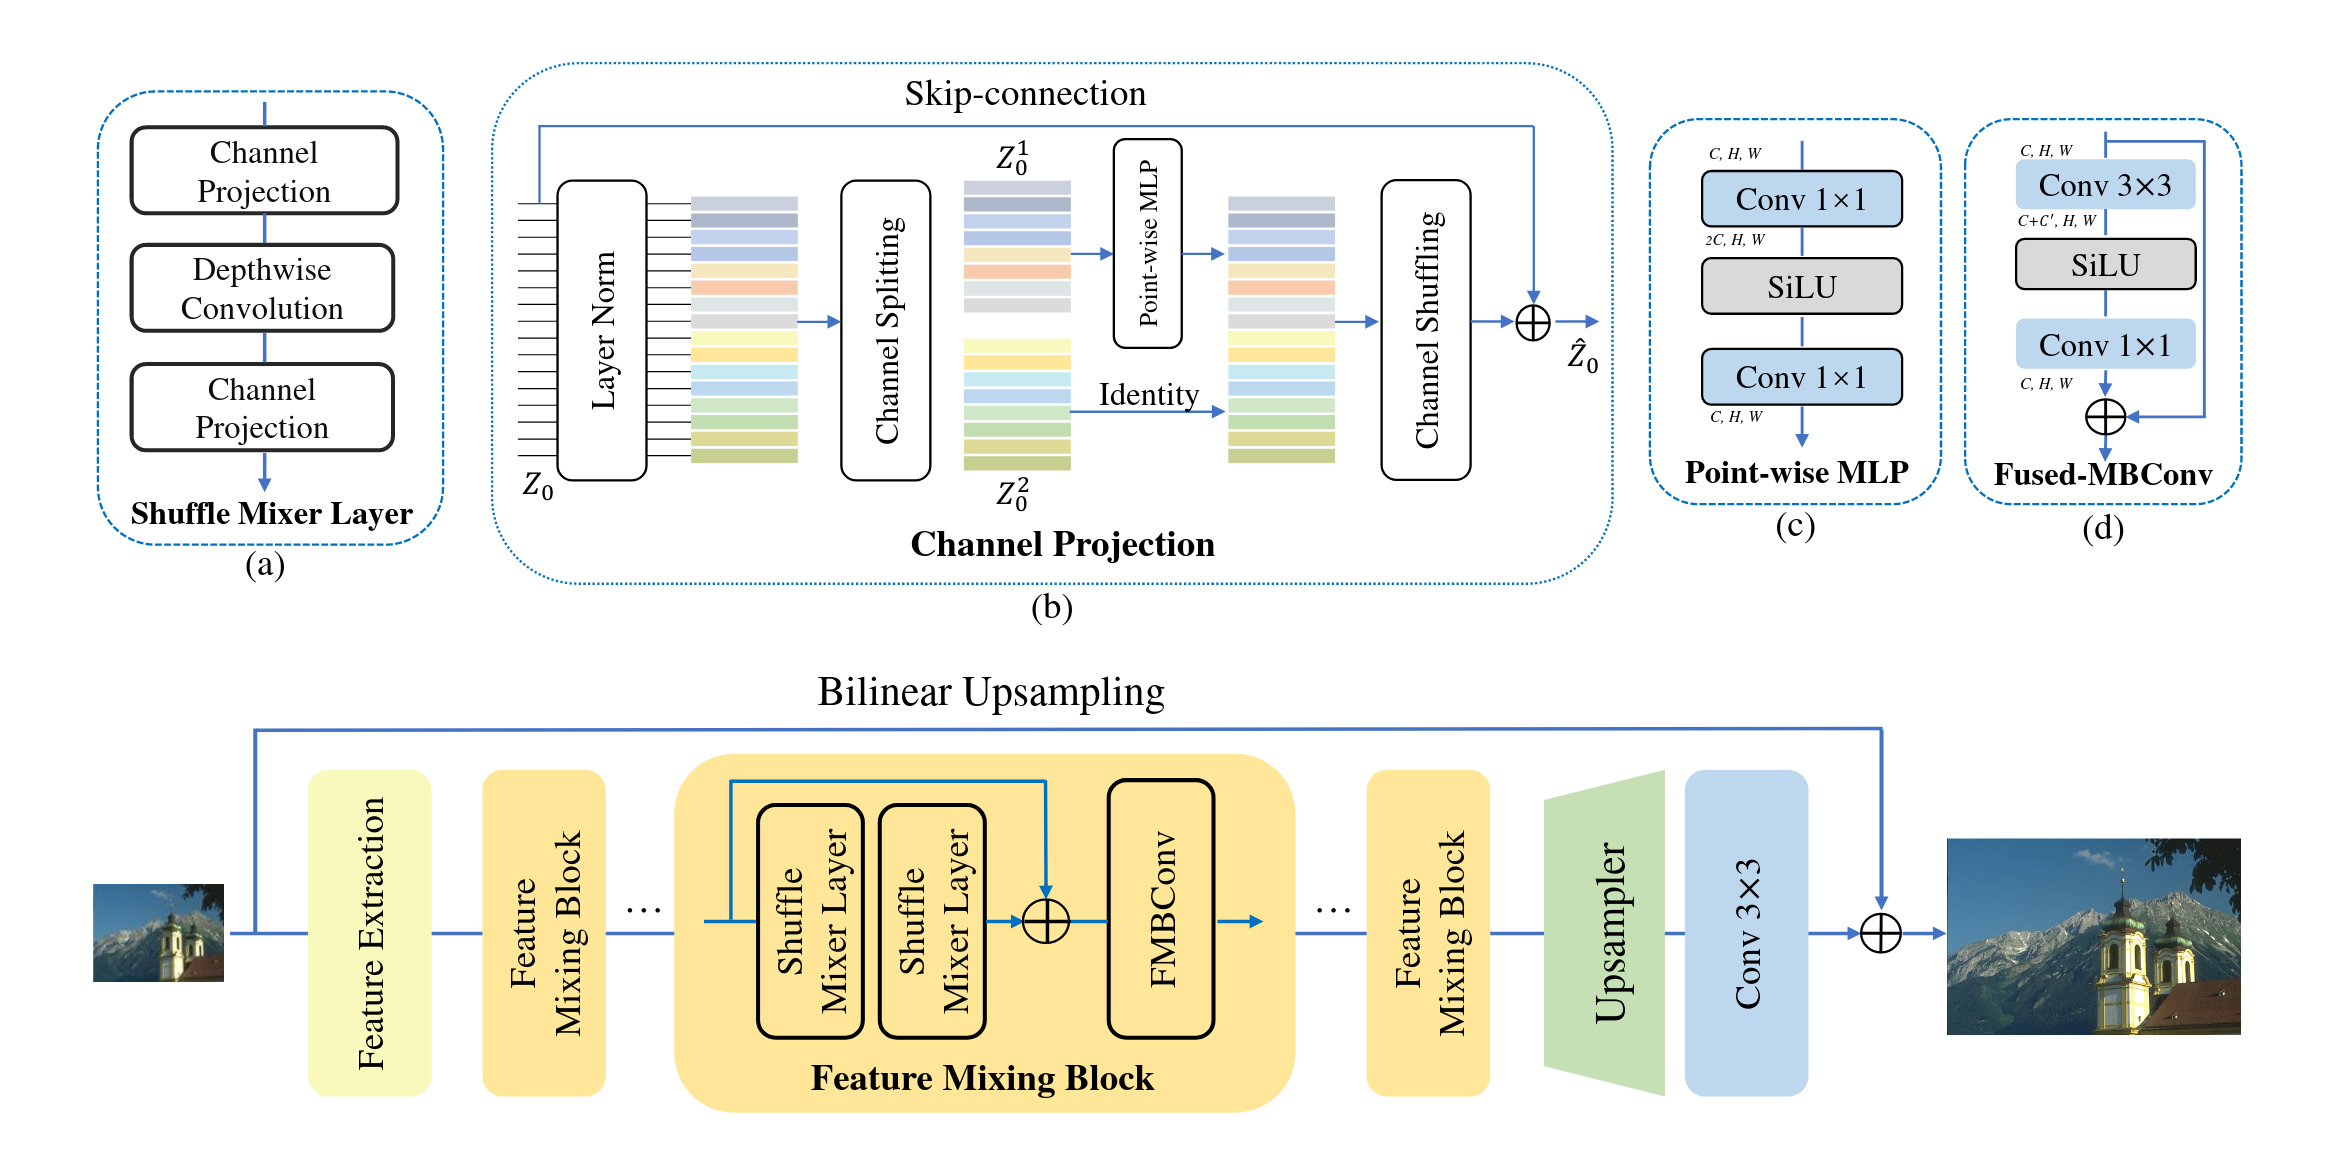
\includegraphics[width=\textwidth]{block diagram.png}
    \caption{Block diagram showing the structure of ShuffleMixer, from \citet{sun2022shufflemixer}.} \label{fig:original_block_diagram}
    \end{figure}

    This figure was used to organize the reimplementation; each block is written as a PyTorch module. For example, the {\em Shuffle Mixer Layer} is shown to include two {\em Channel Projection} blocks with {\em Depthwise Convolution} in between. In a separate section of the figure, the `Channel Projection' block is broken down. So, the {\tt ShuffleMixerLayer} module includes two {\tt ChannelProjection} modules.

    This makes it easy to quickly confirm that the reimplemented architecture is as described in the paper. A number of details are spread out in the text instead, but \cref{fig:original_block_diagram} is complete enough that this is easy to follow. This includes:

    \begin{itemize}
        \item The {\em Feature Extraction} block is a single $3\times3$ convolution layer,
        \item $64\times64$ images are used for input during training,
        \item The {\em Feature Mixing Block} is repeated five times,
        \item The {\em Upsampler} is `only a convolutional layer of size $1\times1$ and a pixel shuffling layer'.
    \end{itemize}

    The implementation of the {\em Depthwise Convolution} was based on the definition given in \citet{liu2022convnet}, which is that depthwise convolution is a group convolution with a number of groups equal to the number of input channels.

    \subsection{Implementation Issues} \label{sec: imp issues}

    A number of issues were encountered while reimplementing ShuffleMixer. They are listed here, along with how they were handled.

    \paragraph{Channel Shuffling Implementation} The model uses a channel shuffling layer, from \citet{zhang2017shufflenet}. PyTorch includes an implementation of channel shuffling, but it doesn't current support auto-differentiation. There is an open issue discussing this on the PyTorch repository \citep{PytorchChannelShuffleIssueGithub}. A different implementation was taken from \citet{KuangliuGitHub}.

    \paragraph{Channel Splitting Ratio} For the channel splitting operation, no ratio was explicitly given in the paper. In \cref{fig:original_block_diagram}, and in the original definition of the operation \citep{ma2018shufflenet}, an equal split is used and so this was chosen.

    \paragraph{Missing Parameters \& Ambiguity} The number of features extracted by the feature extraction layer and the depthwise convolution kernel size are not clearly given in the paper. The following quote is extracted from a section of the paper describing the difference between ShuffleMixer and ShuffleMixerTiny:

    \begin{quotation}
    The number of channels and convolution kernel sizes is 64 and
    $7 \times 7$ pixels for the ShuffleMixer model and 32 and $3 \times 3$ pixels for the ShuffleMixer-Tiny model
    \end{quotation}

    Which can be mapped on to the aforementioned missing parameters. However, this is rather ambiguous; there are many convolutional layers in the model that the above values could be assigned to. Their meaning had to be inferred.

    \paragraph{Padding} A sanity check of the structure was done with TorchInfo and unexpected shapes were found. This was a padding issue, and quickly resolved.

    \paragraph{FFT Parameters} The paper gives a loss function that includes the Fast Fourier Transform, but no parameters are given. As the data is two-dimensional, PyTorch's {\tt fft2} was used with default arguments.

    \paragraph{Datasets} The dataset the original was trained on is DF2K, which is a combination of the high resolution images from DIV2K \citep{Agustsson_2017_CVPR_Workshops} and Flickr2K. No reference could be found for Flickr2K, the reference for it in the original paper \citep{DBLP:journals/corr/LimSKNL17} only mentions DIV2K. There is an issue for this on GitHub, \citet{LimbeeGithub}, but the links given as a solution no longer work. A copy of the dataset was eventually found at \citet{Ddlee_2019Dataset}.

    \subsection{Comparison with Original}

    Before training the new implementation, considering some of the issues above, it made sense to sanity check against the original code. Major differences would indicate that the model cannot be implemented just from the literature. 

    Unfortunately, their implementation does not perfectly follow the block structure from \cref{fig:original_block_diagram}. This isn't surprising as a number of the conceptual blocks are very simple and can be merged without decreasing code readability. An extreme example is {\tt FeatureExtraction}, which does not really need to be a separate module as it contains just one layer. 

    This did make comparing the models slightly more difficult. As an example, the {\em Layer Norm} and concatenation are split from the {\em Channel Projection} equivalent in the original code, and happen directly inside their {\tt SMLayer}. However, it seems that the overall architectures are identical.

    The parameters mentioned in \cref{sec: imp issues} can all be confirmed as correct. This is the splitting ratio, the depthwise kernel size and number of features. That the loss function uses {\tt fft2} can also be confirmed.

    There are some differences, however. Their code also supports x3 scaling, which isn't mentioned the paper. This doesn't affect the x4 model this report examines.

    The only affecting difference is that their {\em Upsampler} finishes with a SiLU layer, counter to the quote given earlier in \cref{sec: reimpl}. This change was carried over to the reimplementation.

    \subsection{Training}

     The original model was trained on a V100, with batches of 64. Neither Iridis 5's Lyceum cluster nor the authors' personal desktops could handle batches of 64, $64 \times 64$ images along with their $256 \times 256$ expected values. Through experimentation, the batch size was reduced to 16.

    The training required loading very large images and cropping random $256 \times 256$ sections. The $256 \times 256$ images are augmented by rotation and flipping, before being downsampled to $64 \times 64$. 
    
    Using a PyTorch {\tt ImageFolder} data loader, followed the necessary transformations, resulted in extremely slow training. A preprocessing script was written to 4x downsample the original dataset, and a custom data loader was written to load those images and perform the same transformations on both. This halved the training time.

    The remaining bottleneck is loading the images themselves. A potential, unimplemented, solution would be to change the images to bitmaps, so that the cropped sections could be streamed from the disk rather than loading the whole image. 

    With the bottleneck being the image loading, there was little difference between training on Iridis and the authors' desktops so the training was done locally. The model was trained for 350,000 iterations (taking about 3 days). This is higher than the original implementation's 300,000 iterations, but the number of examples is lower because of the smaller batch size. 

    \section{Testing}

    Examples from the datasets Celeb A HQ \citep{liu2015faceattributes} and Kitti \citep{Geiger2012CVPR} are included in \cref{example output celeb,example output kitti} respectively. These are the first images of those datasets, so not handpicked. Neither of the models were trained on these datasets, and the datasets were chosen specifically because their content is very different: human faces, and outdoor scenes

    In both cases, there is a gradual improvement from bicubic upsampling, to the  reimplemented model, to the pretrained model. This is most noticeable in areas with straight lines and high contrast. For \cref{example output celeb} this is the teeth, eyelashes and hair, and for \cref{example output kitti} this is the shadows and the buildings. The roof of the building on the right is straight in both of the model outputs, but pixelated for the bicubic upsampling. Important, this improvement can be also seen in the examples shown in the original paper. \Cref{fig:original_output} is one such example, and shows that ShuffleMixer is much better than bicubic upsampling at defining the gaps between pavement tiles.
    
    It makes sense that the pretrained model is better than the reimplemented one as it has seen almost 4x as many examples. It is clear, however, that ShuffleMixer works better than bicubic upsampling on a variety of (new) data, and that so does the reimplemented version.

    \begin{figure}
        \centering
        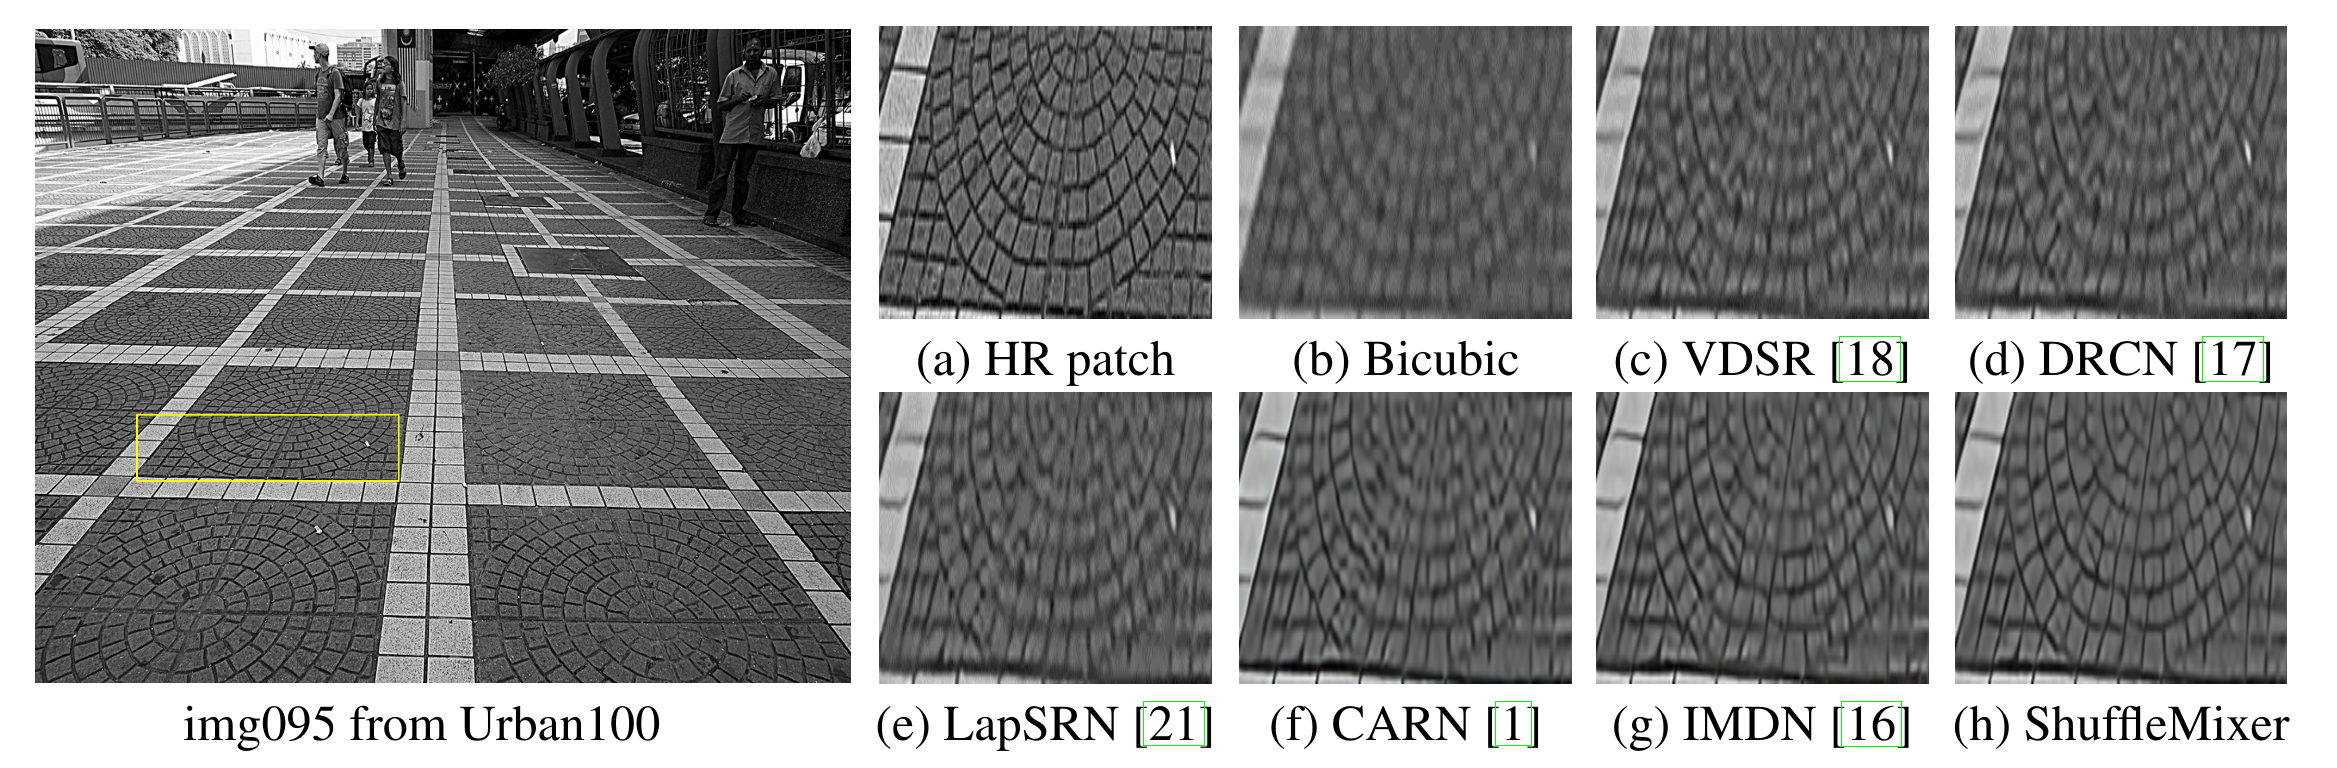
\includegraphics[width=0.55\textwidth]{pavement.png}
        \caption{Examples output generated by ShuffleMixer and competitors, from \citet{sun2022shufflemixer}.} \label{fig:original_output}
    \end{figure}
    
    \section{Analysis}

    \Cref{fig:original_block_diagram} does a lot of heavy lifting when it comes to reimplementing, and therefore reproducing, ShuffleMixer. There were a few issues around vague parameters, but the correct information could all be inferred from the paper even when not explicitly stated. The exception being the missing SiLU layer. However, it isn't unreasonable to expect a reader to assume that a convolutional layer uses the same activation function as every other such layer in the model, not a linear one.

    The fact that the pretrained model produced output that was superior, in a similar way to \cref{fig:original_output}, to bicubic upsampling indicates that the model handles new images well. The fact that the reimplemented model produced similar output to the pretrained model is a strong indicator of the reproducibility of ShuffleMixer.

    Perhaps the final point related to reproducibility is the issue related to obtaining the dataset, the need to download it from a third party. There is no reason that a different dataset couldn't be used however, as long as it had the same variety and was at least the same size.

    Overall, the investigation in this report indicates a high level of reproducibility. Both of the target questions given in \cref{sec:target questions} (and both (1) and so (2) for the second question) can be answered with a strong yes.


    \bibliography{main}
    \bibliographystyle{iclr2022/iclr2022_conference}

    \newpage

    \appendix

    \section{Example Images}
    \begin{figure}[H]
        \centering
        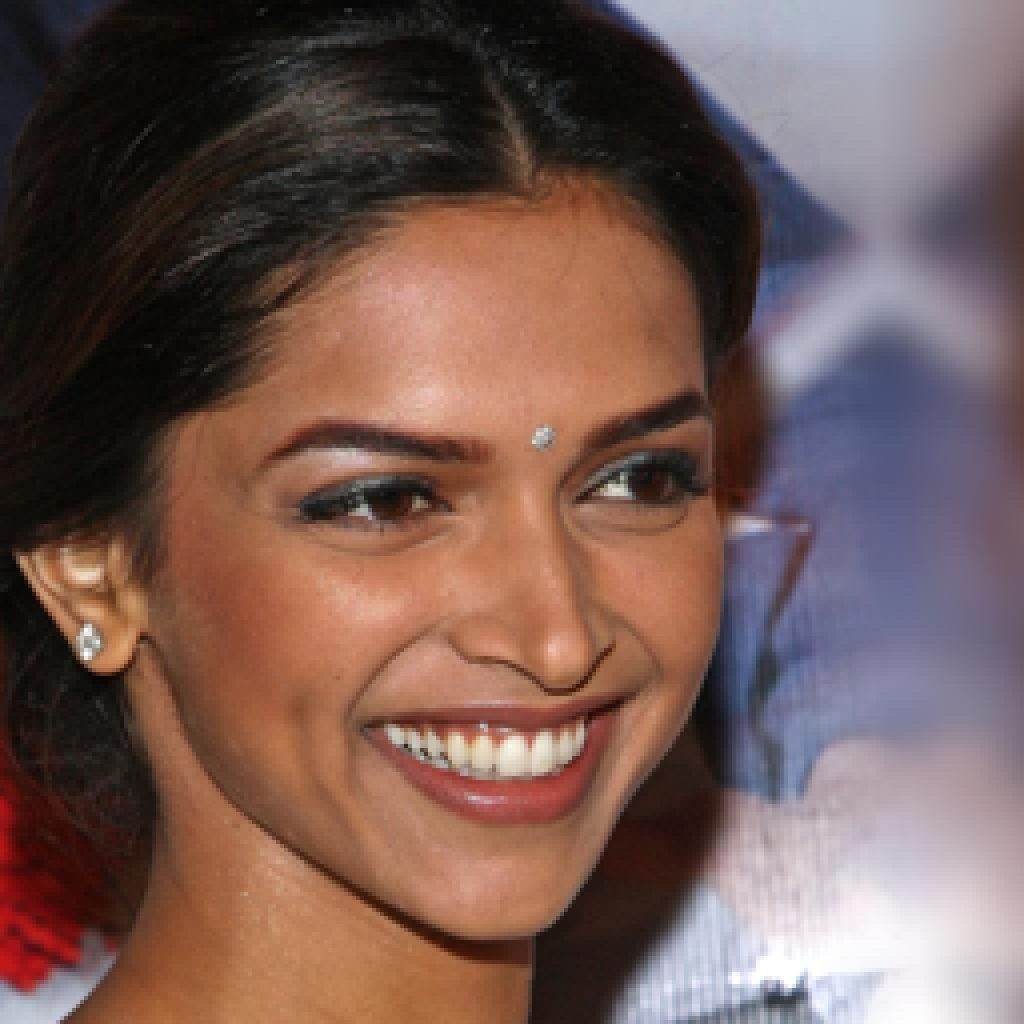
\includegraphics[width=0.4\textwidth]{test_output/nearest celeb_a_hq.png}
        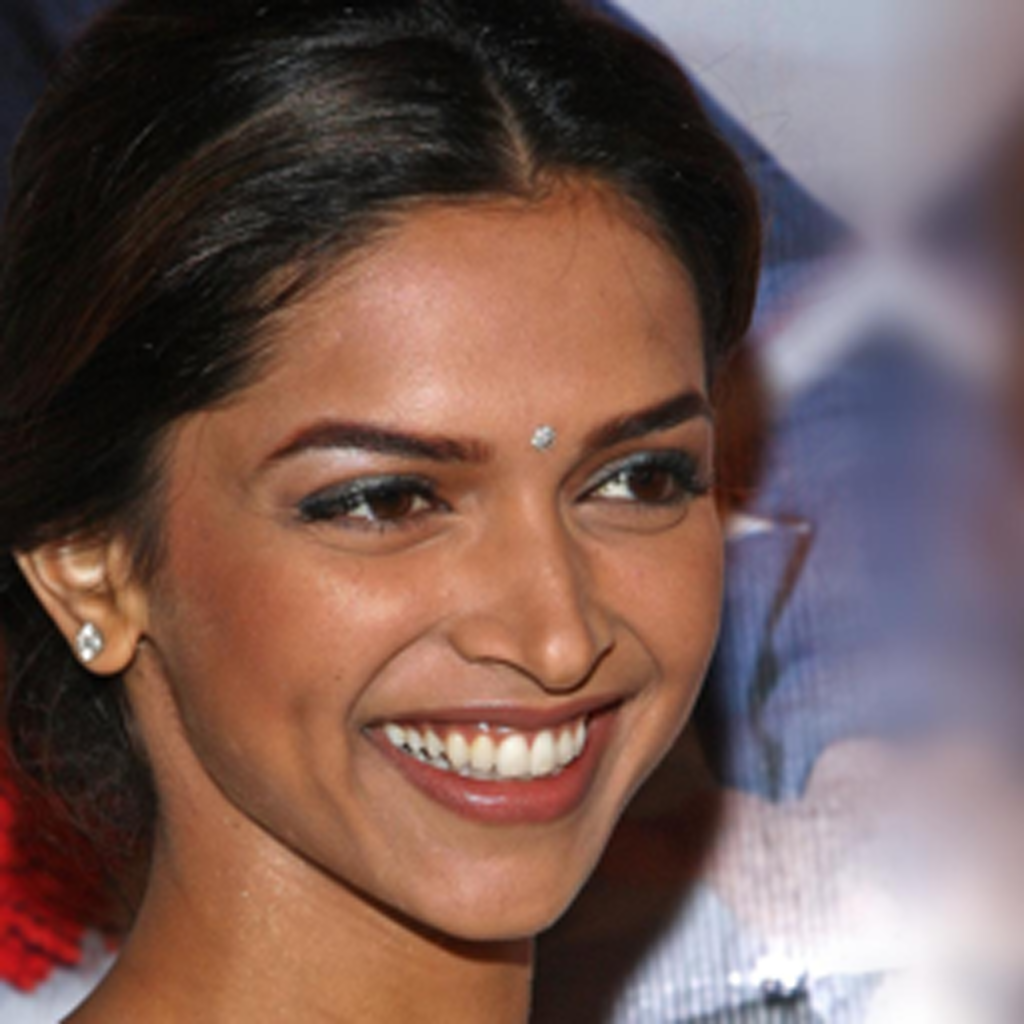
\includegraphics[width=0.4\textwidth]{test_output/bicubic celeb_a_hq.png}
        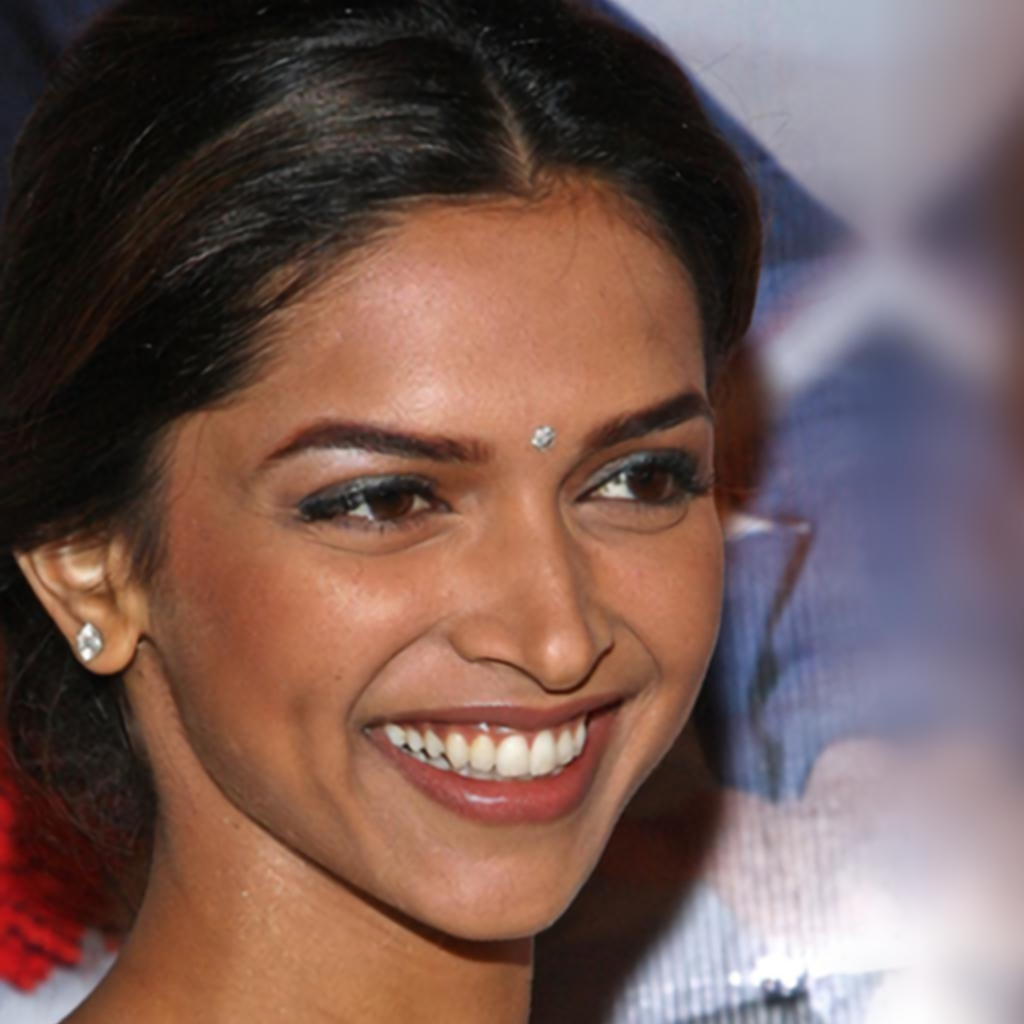
\includegraphics[width=0.4\textwidth]{test_output/model celeb_a_hq.png}
        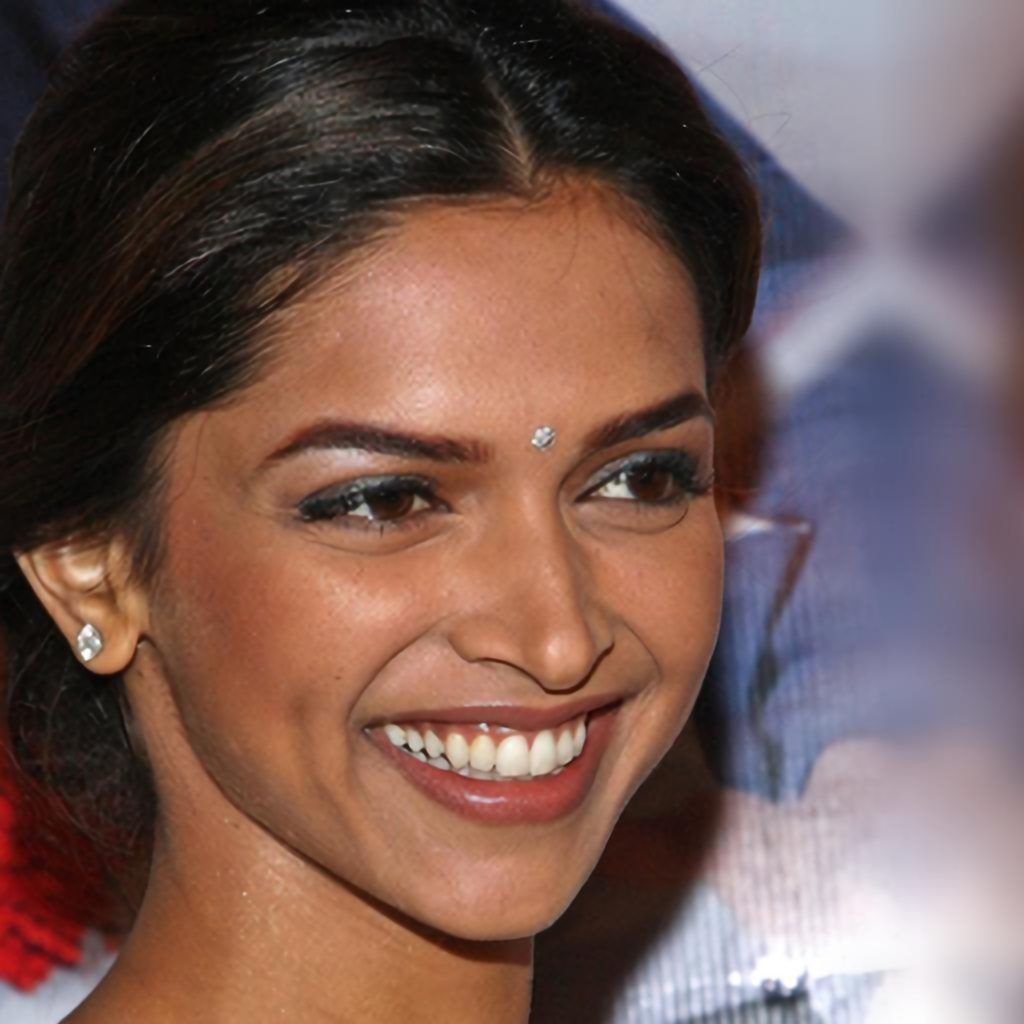
\includegraphics[width=0.4\textwidth]{test_output/pretrained celeb_a_hq.png}
        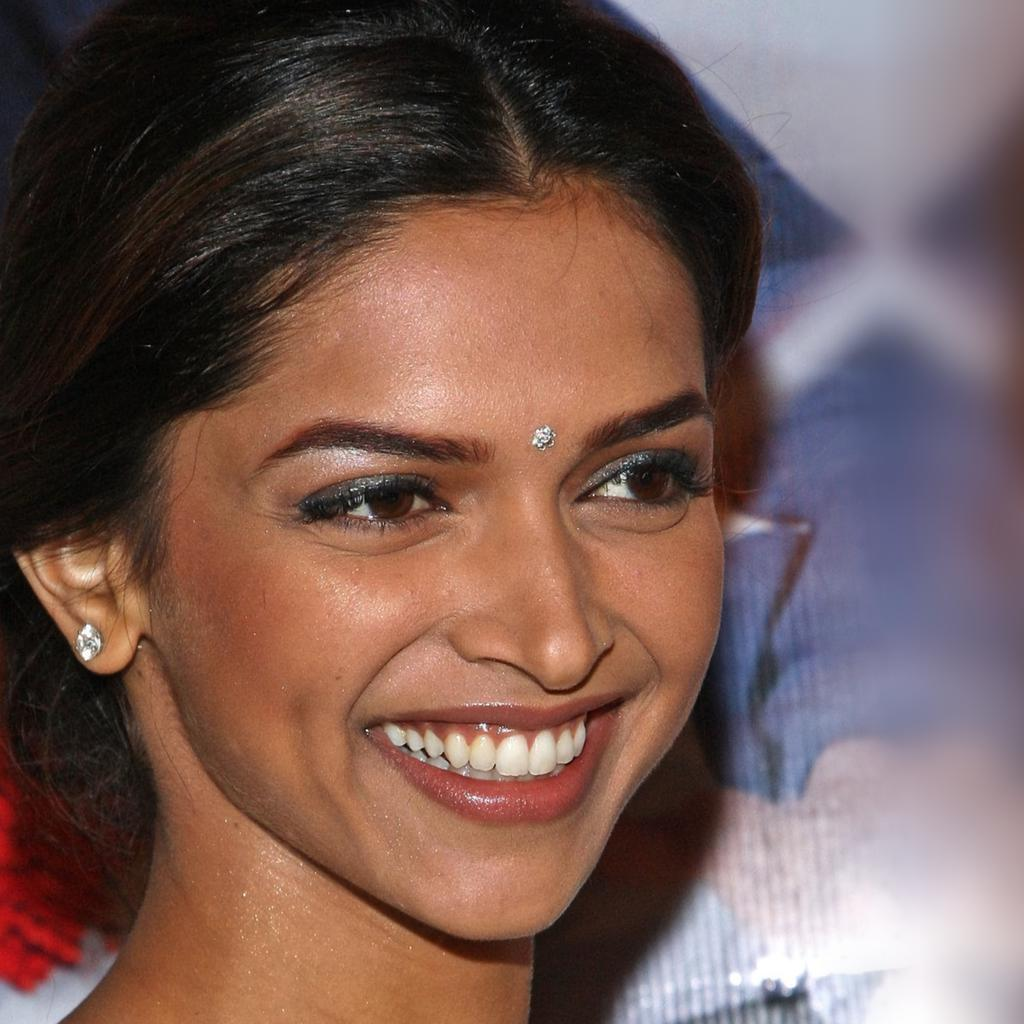
\includegraphics[width=0.4\textwidth]{test_data/celeb_a_hq.png}
        \caption{Example images from the first image in the Celeb A HQ dataset (CITE). The original image (source: \citet{liu2015faceattributes}) is at the bottom, and the image at the top left is it 4x bicubic downsampled. Then, the top-right, mid-left and mid-right are the output of: 4x bicubic upsampling, the reimplemented model, and the pretrained model respectively.} \label{example output celeb}
    \end{figure}

    \begin{figure}
        \centering
        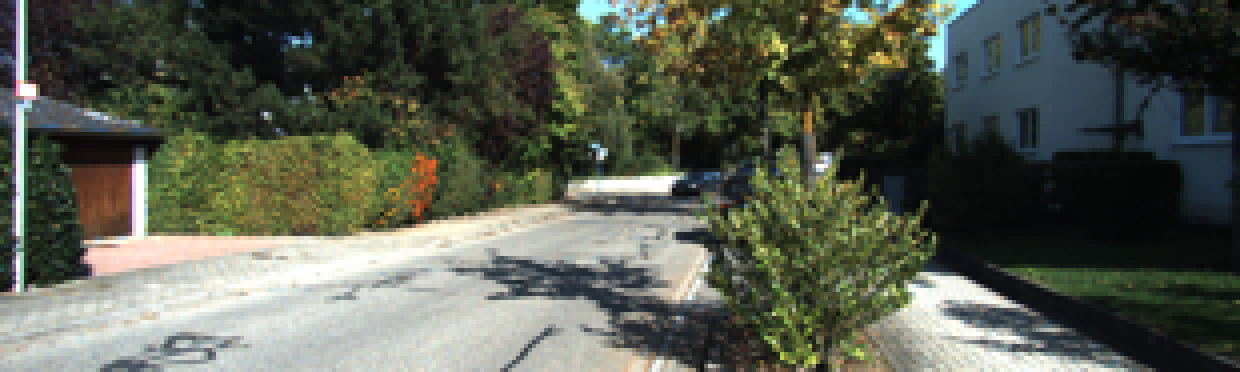
\includegraphics[width=\textwidth]{test_output/nearest kitti.png}
        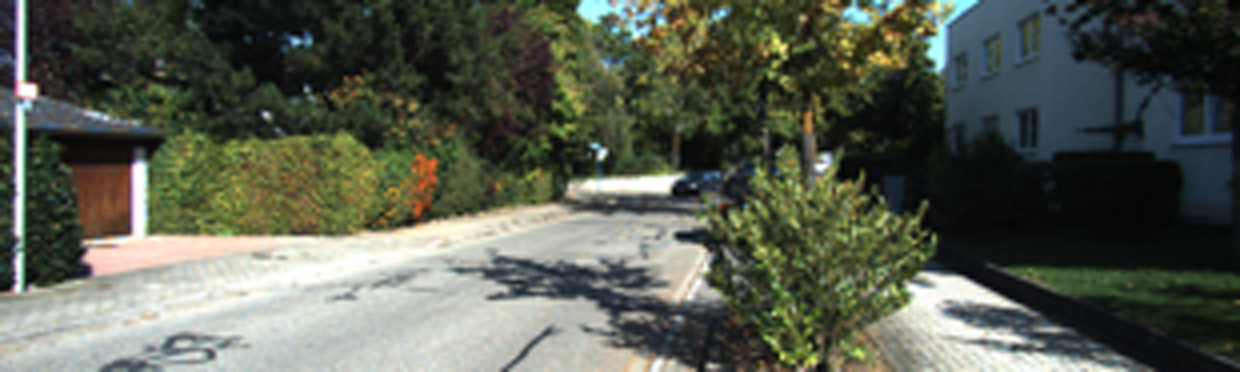
\includegraphics[width=\textwidth]{test_output/bicubic kitti.png}
        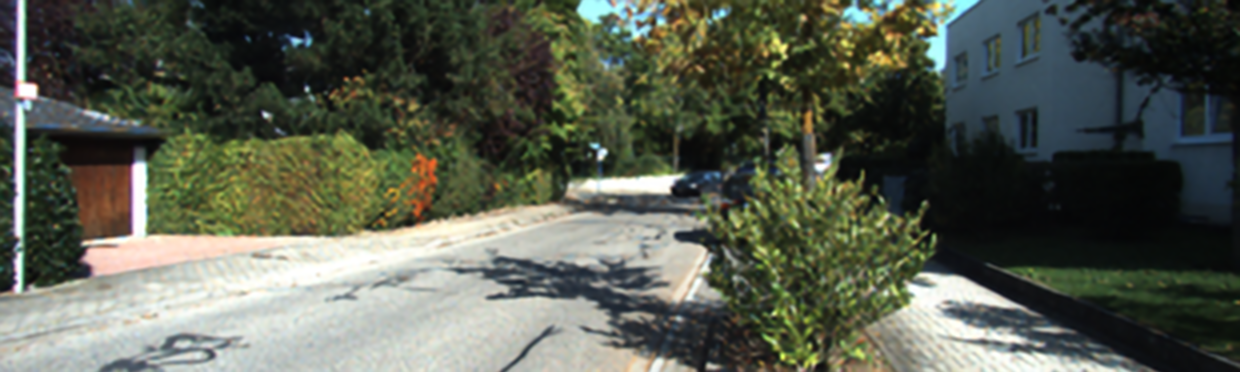
\includegraphics[width=\textwidth]{test_output/model kitti.png}
        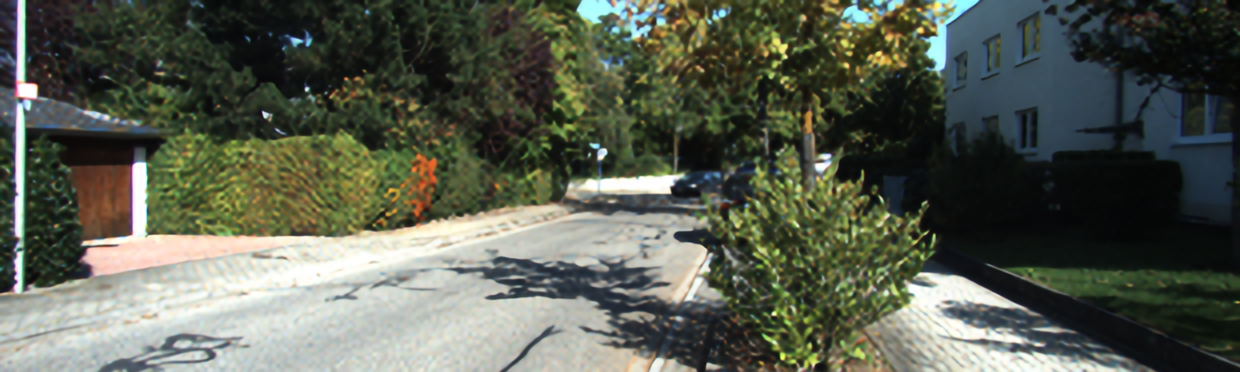
\includegraphics[width=\textwidth]{test_output/pretrained kitti.png}
        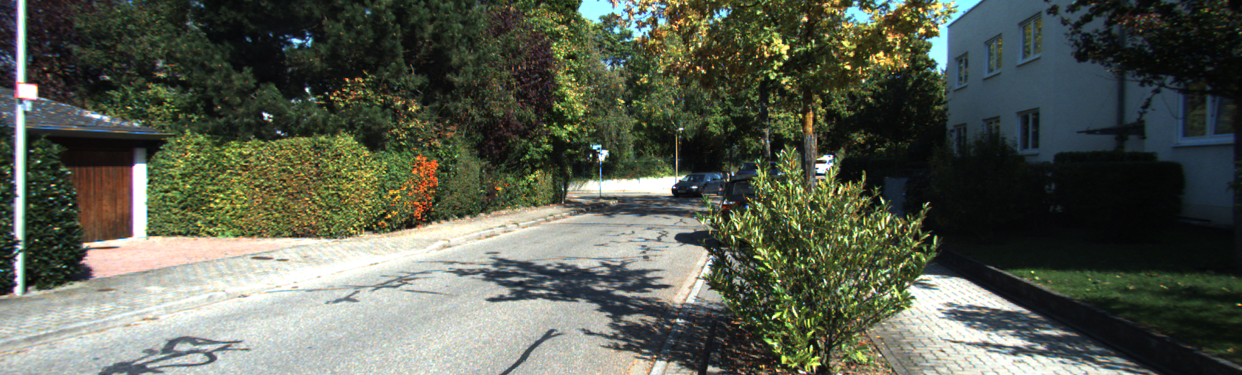
\includegraphics[width=\textwidth]{test_data/kitti.png}
        \caption{Example images from the first image in the Kitti dataset (CITE). The original image (source: \citet{Geiger2012CVPR}) is at the bottom, and the image at the top is it 4x bicubic downsampled. Then, from top to bottom, the remaining images are the output of: 4x bicubic upsampling, the reimplemented model, and the pretrained model.} \label{example output kitti}
    \end{figure}




\end{document}